\documentclass[oneside]{article}
\usepackage{fancyhdr}
\usepackage{graphicx}
\usepackage{float}
\usepackage{enumitem}
\usepackage{listings}
\pagestyle{fancy}
\title{Parallel Design Patterns II}
\author{B138813}
\date{February 2019}

\begin{document}
\lhead{Parallel Design Patterns II}
\rhead{B138813}

\maketitle
\section{Introduction}
We present our report for the second submission of the Parallel Design Patterns Coursework. We first discuss our implementation in Section~\ref{sec:imp}, and demonstrate its correctness in Section~\ref{sec:cor}. Although our implementation has some features similar to a framework, we were not able to succesfully seperate policy and mechanism to an adaquete extend. We will discuss this issue further in Section~\ref{sec:fur}.



\section{Implementation}\label{sec:imp}
We implemented our squirrel simulation in C++. We present a UML diagram of our implementation in Figure~\ref{fig:uml}. To maximise code re-use, and to conform to the actor pattern, we abstracted as much common functionality into the parent actor class as possible. Every object in the actor pattern must be an actor, so we every class inherits from the actor class. The actor class holds methods such as \texttt{send\_msg()} and \texttt{msg\_recv()} which act as wrappers to MPI functions, whilst also providing extra functionality. For example, \texttt{msg\_recv()} returns a three item tuple, which contains:

\begin{itemize}
  \item A boolean, which indicates if the message was succesfully recieved.
  \item An integer, which indicates where the message was recived from.
  \item An integer, which is the message itself.
\end{itemize}
The semantics of the message integer are encoded into the \texttt{MSG} enum, which is shared by all actors. This standardisation makes it easy for the programmer to reason about messages, allowing them to dictate how a message if handled in each child class's main event loop. The function \texttt{send\_msg()} is simple convenience wrapper around \texttt{MPI\_Bsend()}. Each class inherits directly from the actor class, except for the controller, which is a child of the master class. We made this decision because the master and controller share most of their functionality and variables. The master class starts the simulation, and then provides process pool functionality. The controller class keeps track of the number of live and infected squirrels.

\begin{figure}[H]
  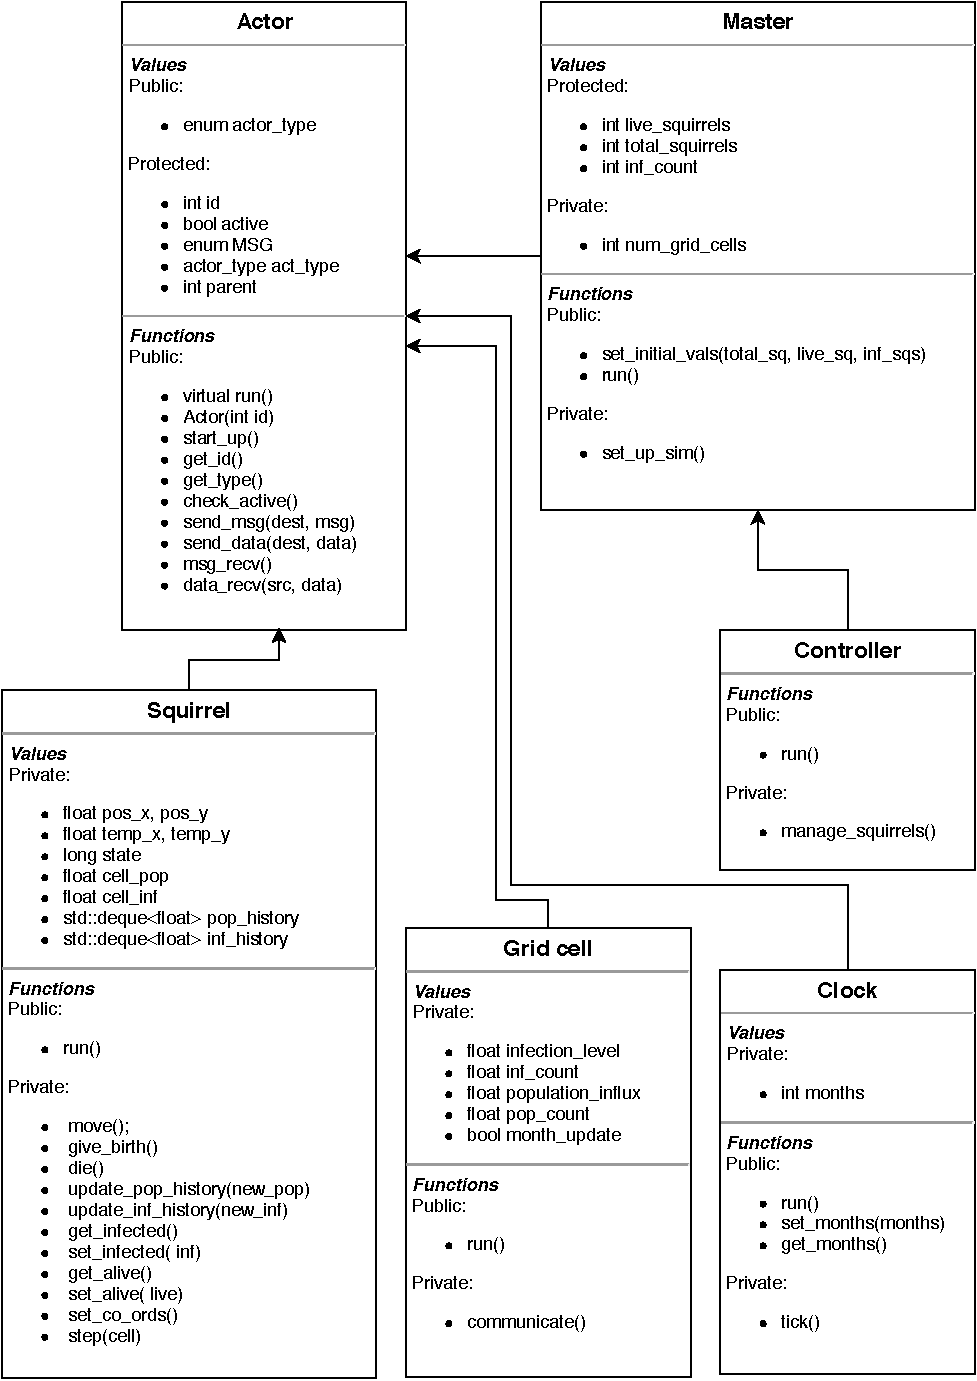
\includegraphics[width=\linewidth]{figures/pdp_uml}
  \caption{UML Diagram of the Program}
  \label{fig:uml}
\end{figure}
It also mediates the birth of squirrels after the master has set up the simulation. There is only ever one controller and one master. Both classes need to know the simulation's initial squirrel numbers, and share functions and values to implement this. If C++'s inheritance model did not allow both child and grandchild classes to implement their own versions their parent's virtual functions, this pattern would not be possible. The squirrel class uses the squirrel functions provided to us by the biologists, which results in it having the most functions of any class. Another reason the squirrel class has so many functions is of how we have decided to model our actor types.

 Each actor has an actor type, as designated by the enumerate type \texttt{actor\_type}. There three different actor type for squirrels; infected squirrels, dead squirrels and normal, healthy squirrels. To safely change a squirrel from one of these types to another, we thought it best to encapsulate the code within a function. In doing so, we keep our code compliant with object oriented design philosophies, but diverge from high performance programming ones. However, we do not think the addition of these functions degrades the performance of our work too much, and improves the readablity of our code.

 There are four key communications between our actors. We have endevored to abstract them and encapulate them into our actor class. We will now describe our implementations of those actors. It is important to note that we never use blocking sends. If we want to be sure that a certain actor receives a message before it continues, we use a blocking receive. Unless otherwise stated, all receives are non blocking.

 \subsection{Actor Start}
 Every actor except master enters into the worker code function and calls \texttt{start\_up()}, where the actor uses a blocking recieve to get what type of actor it is from the master. Once the actor has recieved its type, it can begin to execute its \texttt{run()} function, where its behavior is encapsulated in a \texttt{while(active)} loop. It is important that the grid cells and the controller are created in the order that they are, as communication is reliant up their ranks being between 1 and 16 for squirrels, and exactly 17 for the controller. Squirrels, unlike all other actors, must use one more blocking recive before entering this loop, which we will go onto explain in the next section.
\subsection{Squirrel Birth}
Before a squirrel can enter its \texttt{while(active)} it must first be assigned its co-ordinates. This therefore means that the squirrel must use a blocking recieve to gather its co-ordinates from either the master, or the controller, depending on which actor started it.

When a squirrel gives birth to another squirrel it sends a message to the controller to inform it that it is giving birth. Once the controller has recieved this message, it uses a blocking recieve to get the location vector of the squirrel. After receiving that location vector, the controller starts a new worker process, and sends on the location vector it has just received.
\subsection{Squirrel Step}
Every time a squirrel steps into a grid cell, each must exchange key statistics about infection and population. To ensure that a squirrel has stepped into a grid cell and succesfully retrieved data from it, the squirrel's \texttt{step()} function returns a boolean indicating if the squirrel recieved the population influx and infection level from the grid cell. If the returned boolean is false, then the squirrel does not carry out the rest of its functionality, because its most recent value for a cell's population influx and infection level would be inacurrate. The biologist's model mandates a strong relationship between the squirrel and the enviroment, so we must remain faithful to that.

A grid cell's side of this communication is much simpler, only incrementing its population count or population and infection count when a squirrel sends a step or an infected step respectively.
\subsection{Clock tick}
We have made use of a clock actor to send messages to every grid cell each month, modelled as a period of 0.05 seconds. We refer to this time period message as a tick. Both the grid cell and the controller's \texttt{run()} receive tick messages. When the grid cell receives a tick, it updates its population influx and infection level in accordance with the biologist's model. Although a grid cell does not have a particulalry long history of population or infection counts, we have decided to model the history as a FIFO deque. This allows us to use familliar pop back and push front conventions to maintain the size of the history. Although this is perhaps not the most performant way to manage the history of the of the grid cells, we hope that it's familiarity makes it easier to maintain. We also use the same method to manage the squirrels infection level and recent population history.

If the controller recieves a message from the clock it prints out the current number of live squirrels and the number of dead squirrels.

\section{Correctness}\label{sec:cor}
Although our we embrace the chaotic nature of the actor pattern and the model we are simulating, we can still demonstrate the correctness of our implementation. For example, if there are no infected squirrels at the start of the simulation, then the number of squirrels will reach 200 and force the simulation to end. Simililarly, if we set the number of infected squirrels to be equal to the initial number of squirrels, the squirrels will all die, causing the simulation to end early.

Our program will routinely give similar output for the same initial parameters. For example, we found that with suggested parameters the simulation stays in a steady state, begining with 34 live squirrels and ending with 34 $\pm$ 2. Although the simulation starts with 4 infected squirrels, we found that the number of infected squirrels in the simulation printed by the controller actor each month rapidly approached zero, and would only sometimes increase to one. We believe this is because it takes a squirrel less than a month to die after being infected.

We include a sample output in Appendix~\ref{sec:sample}, which we have graphed into Figure~\ref{fig:prog-ex}. In this figure, the values of average population and average infection are taken from all of the grid cells population influx and infection level at monthly intervals. The live and infected squirrel values are reported to us by the controller actor, also after each month. We have included the python script used to generate the csv file this figure is generated from in the code submission.
\begin{figure}
  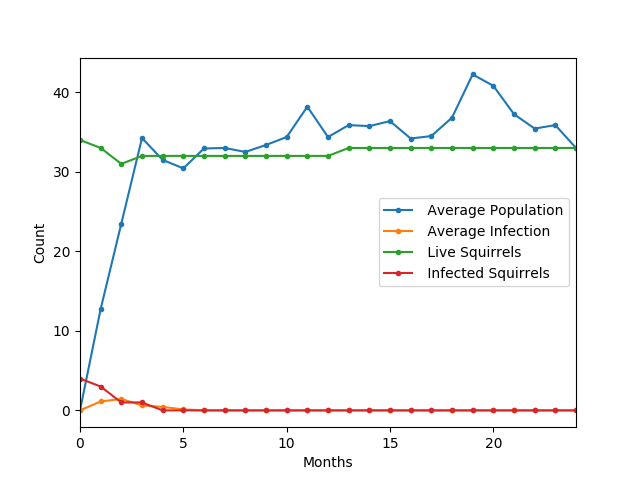
\includegraphics[width=\linewidth]{figures/d1}
  \caption{Stastics from Program Execution}
  \label{fig:prog-ex}
\end{figure}

Our graph's visualisation of the output data validates our claim of correctness, insofar as it proves a correspondance between the number of live squirrels and the average population value, and between the number of infected squirrels and the average infection level.

\subsection{Issues}
Our solution is not portable. The outcome of the simulation is highly dependant on the speed of the processor which runs it, as on faster processors the squirrel moves faster, increasing the average population value to such a level that new squirrels are unlikely to be born. To fix this issue would require us speaking to the biologists to adjust their model, or working to make the number of steps per month always fall within a certain range.

When there are a high number of live squirrels, the controller and grid cell actors become too busy to recieve clock ticks. We found that more with more than 150 squirrels, we were unlikely to recieve any information from either the controller or the grid cell actors. We are unsure of how to resolve this, but the answer could lie in making multiple controller actors, who at month intervals would message a single counter actor. We could also reduce traffic to the controller by allowing squirrels to spawn their own processes, and only messaging the controller that they have given birth, rather than passing over their location. However, this solution will not aid our grid cell actors to receive clock ticks.

\section{Further Work}\label{sec:fur}
Our work does contain some of the foundations of a framework within it, and we would hope to develop these foundations in any further work. Our \texttt{send\_msg()} and \texttt{msg\_recv()} methods are adaquete for a framework, in that they cope with the mechanism for the programmer and allow them to implement their own policy on how messages should be dealt with when received.  Whilst we do have a general data recieve method, it is not general enough for all of our use cases, such as when we need to do a blocking receive before moving on with our processing. As MPI garuntees that messages are recieved in the order they are sent in, we could easily implement sending and recieving location data as a combination of blocking messages, one for each co-ordinate.

If we were to implement a framework, it we would simply require that people inherit from our actor class to use its methods and conform to its usage requirements. A key difference between our imagined framework and our actual implementation is that our framework would restrict all MPI code to the actor class. We would also like to use C++'s powerful templating and traits to allow us to generalise our send a recives so that the programmer using the framework could call \texttt{send\_data()} without having to be concerned about the data type they were sending.

\appendix
\section{Sample Output}\label{sec:sample}
\begin{lstlisting}[basicstyle=\tiny]
Master 0: Creating sim with 34 squirrels, of which 4 are infected
gc 1: month: 1 population_influx: 12.000000 infection_level: 0.000000
gc 3: month: 1 population_influx: 10.000000 infection_level: 5.000000
gc 5: month: 1 population_influx: 13.000000 infection_level: 0.000000
gc 6: month: 1 population_influx: 12.000000 infection_level: 0.000000
gc 7: month: 1 population_influx: 11.000000 infection_level: 2.000000
gc 9: month: 1 population_influx: 12.000000 infection_level: 0.000000
gc 10: month: 1 population_influx: 12.000000 infection_level: 1.000000
gc 11: month: 1 population_influx: 17.000000 infection_level: 0.000000
tick 1
C17: month: 1 live_squirrels: 33 infected: 3
gc 4: month: 1 population_influx: 13.000000 infection_level: 2.000000
gc 14: month: 1 population_influx: 13.000000 infection_level: 0.000000
gc 13: month: 1 population_influx: 13.000000 infection_level: 1.000000
gc 15: month: 1 population_influx: 15.000000 infection_level: 0.000000
gc 2: month: 1 population_influx: 10.000000 infection_level: 1.000000
gc 8: month: 1 population_influx: 17.000000 infection_level: 2.000000
gc 12: month: 1 population_influx: 18.000000 infection_level: 1.000000
gc 16: month: 1 population_influx: 6.000000 infection_level: 3.000000
gc 1: month: 2 population_influx: 21.000000 infection_level: 0.000000
gc 3: month: 2 population_influx: 20.000000 infection_level: 5.000000
gc 5: month: 2 population_influx: 20.000000 infection_level: 0.000000
gc 7: month: 2 population_influx: 17.000000 infection_level: 3.000000
gc 10: month: 2 population_influx: 27.000000 infection_level: 2.000000
gc 16: month: 2 population_influx: 15.000000 infection_level: 3.000000
tick 2
C17: month: 2 live_squirrels: 31 infected: 1
gc 4: month: 2 population_influx: 27.000000 infection_level: 2.000000
gc 13: month: 2 population_influx: 21.000000 infection_level: 1.000000
gc 6: month: 2 population_influx: 24.000000 infection_level: 2.000000
gc 15: month: 2 population_influx: 21.000000 infection_level: 0.000000
gc 2: month: 2 population_influx: 27.000000 infection_level: 1.000000
gc 12: month: 2 population_influx: 32.000000 infection_level: 1.000000
gc 8: month: 2 population_influx: 31.000000 infection_level: 2.000000
gc 14: month: 2 population_influx: 22.000000 infection_level: 0.000000
gc 9: month: 2 population_influx: 24.000000 infection_level: 0.000000
gc 11: month: 2 population_influx: 27.000000 infection_level: 1.000000
gc 1: month: 3 population_influx: 31.000000 infection_level: 0.000000
gc 3: month: 3 population_influx: 31.000000 infection_level: 0.000000
gc 7: month: 3 population_influx: 28.000000 infection_level: 1.000000
gc 9: month: 3 population_influx: 34.000000 infection_level: 0.000000
gc 10: month: 3 population_influx: 34.000000 infection_level: 2.000000
gc 15: month: 3 population_influx: 38.000000 infection_level: 0.000000
tick 3
gc 5: month: 3 population_influx: 29.000000 infection_level: 0.000000
gc 4: month: 3 population_influx: 36.000000 infection_level: 0.000000
gc 6: month: 3 population_influx: 36.000000 infection_level: 3.000000
gc 13: month: 3 population_influx: 33.000000 infection_level: 1.000000
gc 2: month: 3 population_influx: 38.000000 infection_level: 1.000000
C17: month: 3 live_squirrels: 32 infected: 1
gc 12: month: 3 population_influx: 44.000000 infection_level: 0.000000
gc 8: month: 3 population_influx: 43.000000 infection_level: 0.000000
gc 11: month: 3 population_influx: 39.000000 infection_level: 1.000000
gc 14: month: 3 population_influx: 27.000000 infection_level: 0.000000
gc 16: month: 3 population_influx: 27.000000 infection_level: 1.000000
gc 1: month: 4 population_influx: 31.000000 infection_level: 0.000000
gc 3: month: 4 population_influx: 28.000000 infection_level: 0.000000
gc 7: month: 4 population_influx: 27.000000 infection_level: 1.000000
gc 8: month: 4 population_influx: 40.000000 infection_level: 0.000000
gc 9: month: 4 population_influx: 34.000000 infection_level: 0.000000
gc 10: month: 4 population_influx: 36.000000 infection_level: 1.000000
gc 14: month: 4 population_influx: 20.000000 infection_level: 0.000000
tick 4
gc 15: month: 4 population_influx: 34.000000 infection_level: 0.000000
gc 4: month: 4 population_influx: 30.000000 infection_level: 0.000000
gc 6: month: 4 population_influx: 33.000000 infection_level: 1.000000
gc 2: month: 4 population_influx: 44.000000 infection_level: 1.000000
gc 13: month: 4 population_influx: 34.000000 infection_level: 2.000000
C17: month: 4 live_squirrels: 32 infected: 0
gc 11: month: 4 population_influx: 26.000000 infection_level: 0.000000
gc 12: month: 4 population_influx: 36.000000 infection_level: 0.000000
gc 16: month: 4 population_influx: 28.000000 infection_level: 1.000000
gc 5: month: 4 population_influx: 23.000000 infection_level: 0.000000
gc 3: month: 5 population_influx: 33.000000 infection_level: 0.000000
gc 5: month: 5 population_influx: 25.000000 infection_level: 0.000000
gc 9: month: 5 population_influx: 33.000000 infection_level: 0.000000
gc 10: month: 5 population_influx: 27.000000 infection_level: 0.000000
gc 14: month: 5 population_influx: 23.000000 infection_level: 0.000000
C17: month: 5 live_squirrels: 32 infected: 0
tick 5
gc 6: month: 5 population_influx: 31.000000 infection_level: 0.000000
gc 2: month: 5 population_influx: 31.000000 infection_level: 0.000000
gc 13: month: 5 population_influx: 36.000000 infection_level: 1.000000
gc 11: month: 5 population_influx: 27.000000 infection_level: 0.000000
gc 15: month: 5 population_influx: 39.000000 infection_level: 0.000000
gc 4: month: 5 population_influx: 26.000000 infection_level: 0.000000
gc 16: month: 5 population_influx: 28.000000 infection_level: 0.000000
gc 12: month: 5 population_influx: 31.000000 infection_level: 0.000000
gc 1: month: 5 population_influx: 31.000000 infection_level: 0.000000
gc 7: month: 5 population_influx: 31.000000 infection_level: 1.000000
gc 8: month: 5 population_influx: 35.000000 infection_level: 0.000000
gc 9: month: 6 population_influx: 40.000000 infection_level: 0.000000
C17: month: 6 live_squirrels: 32 infected: 0
tick 6
gc 2: month: 6 population_influx: 30.000000 infection_level: 0.000000
gc 13: month: 6 population_influx: 32.000000 infection_level: 0.000000
gc 15: month: 6 population_influx: 36.000000 infection_level: 0.000000
gc 11: month: 6 population_influx: 25.000000 infection_level: 0.000000
gc 4: month: 6 population_influx: 27.000000 infection_level: 0.000000
gc 6: month: 6 population_influx: 29.000000 infection_level: 0.000000
gc 16: month: 6 population_influx: 31.000000 infection_level: 0.000000
gc 1: month: 6 population_influx: 35.000000 infection_level: 0.000000
gc 12: month: 6 population_influx: 33.000000 infection_level: 0.000000
gc 7: month: 6 population_influx: 36.000000 infection_level: 0.000000
gc 8: month: 6 population_influx: 34.000000 infection_level: 0.000000
gc 10: month: 6 population_influx: 44.000000 infection_level: 0.000000
gc 14: month: 6 population_influx: 30.000000 infection_level: 0.000000
gc 3: month: 6 population_influx: 39.000000 infection_level: 0.000000
gc 5: month: 6 population_influx: 26.000000 infection_level: 0.000000
gc 2: month: 7 population_influx: 27.000000 infection_level: 0.000000
gc 5: month: 7 population_influx: 28.000000 infection_level: 0.000000
gc 10: month: 7 population_influx: 38.000000 infection_level: 0.000000
gc 13: month: 7 population_influx: 35.000000 infection_level: 0.000000
tick 7
gc 4: month: 7 population_influx: 30.000000 infection_level: 0.000000
gc 9: month: 7 population_influx: 34.000000 infection_level: 0.000000
gc 6: month: 7 population_influx: 27.000000 infection_level: 0.000000
gc 11: month: 7 population_influx: 33.000000 infection_level: 0.000000
gc 15: month: 7 population_influx: 37.000000 infection_level: 0.000000
gc 1: month: 7 population_influx: 31.000000 infection_level: 0.000000
gc 7: month: 7 population_influx: 37.000000 infection_level: 0.000000
gc 3: month: 7 population_influx: 41.000000 infection_level: 0.000000
gc 8: month: 7 population_influx: 31.000000 infection_level: 0.000000
gc 12: month: 7 population_influx: 30.000000 infection_level: 0.000000
gc 14: month: 7 population_influx: 34.000000 infection_level: 0.000000
gc 16: month: 7 population_influx: 35.000000 infection_level: 0.000000
C17: month: 7 live_squirrels: 32 infected: 0
gc 2: month: 8 population_influx: 38.000000 infection_level: 0.000000
gc 5: month: 8 population_influx: 29.000000 infection_level: 0.000000
gc 10: month: 8 population_influx: 43.000000 infection_level: 0.000000
C17: month: 8 live_squirrels: 32 infected: 0
tick 8
gc 13: month: 8 population_influx: 30.000000 infection_level: 0.000000
gc 4: month: 8 population_influx: 31.000000 infection_level: 0.000000
gc 11: month: 8 population_influx: 30.000000 infection_level: 0.000000
gc 6: month: 8 population_influx: 23.000000 infection_level: 0.000000
gc 16: month: 8 population_influx: 38.000000 infection_level: 0.000000
gc 7: month: 8 population_influx: 33.000000 infection_level: 0.000000
gc 1: month: 8 population_influx: 29.000000 infection_level: 0.000000
gc 15: month: 8 population_influx: 32.000000 infection_level: 0.000000
gc 3: month: 8 population_influx: 31.000000 infection_level: 0.000000
gc 8: month: 8 population_influx: 29.000000 infection_level: 0.000000
gc 9: month: 8 population_influx: 33.000000 infection_level: 0.000000
gc 12: month: 8 population_influx: 30.000000 infection_level: 0.000000
gc 14: month: 8 population_influx: 41.000000 infection_level: 0.000000
gc 3: month: 9 population_influx: 26.000000 infection_level: 0.000000
gc 6: month: 9 population_influx: 31.000000 infection_level: 0.000000
gc 8: month: 9 population_influx: 36.000000 infection_level: 0.000000
gc 9: month: 9 population_influx: 32.000000 infection_level: 0.000000
gc 11: month: 9 population_influx: 33.000000 infection_level: 0.000000
gc 12: month: 9 population_influx: 31.000000 infection_level: 0.000000
gc 14: month: 9 population_influx: 43.000000 infection_level: 0.000000
gc 15: month: 9 population_influx: 33.000000 infection_level: 0.000000
tick 9
gc 5: month: 9 population_influx: 26.000000 infection_level: 0.000000
gc 13: month: 9 population_influx: 40.000000 infection_level: 0.000000
C17: month: 9 live_squirrels: 32 infected: 0
gc 10: month: 9 population_influx: 26.000000 infection_level: 0.000000
gc 2: month: 9 population_influx: 45.000000 infection_level: 0.000000
gc 4: month: 9 population_influx: 33.000000 infection_level: 0.000000
gc 16: month: 9 population_influx: 34.000000 infection_level: 0.000000
gc 1: month: 9 population_influx: 28.000000 infection_level: 0.000000
gc 7: month: 9 population_influx: 37.000000 infection_level: 0.000000
gc 8: month: 10 population_influx: 39.000000 infection_level: 0.000000
gc 9: month: 10 population_influx: 32.000000 infection_level: 0.000000
gc 10: month: 10 population_influx: 27.000000 infection_level: 0.000000
gc 11: month: 10 population_influx: 28.000000 infection_level: 0.000000
gc 12: month: 10 population_influx: 37.000000 infection_level: 0.000000
gc 13: month: 10 population_influx: 40.000000 infection_level: 0.000000
gc 14: month: 10 population_influx: 45.000000 infection_level: 0.000000
gc 15: month: 10 population_influx: 35.000000 infection_level: 0.000000
C17: month: 10 live_squirrels: 32 infected: 0
tick 10
gc 3: month: 10 population_influx: 21.000000 infection_level: 0.000000
gc 6: month: 10 population_influx: 34.000000 infection_level: 0.000000
gc 2: month: 10 population_influx: 41.000000 infection_level: 0.000000
gc 4: month: 10 population_influx: 37.000000 infection_level: 0.000000
gc 1: month: 10 population_influx: 33.000000 infection_level: 0.000000
gc 16: month: 10 population_influx: 34.000000 infection_level: 0.000000
gc 5: month: 10 population_influx: 31.000000 infection_level: 0.000000
gc 7: month: 10 population_influx: 36.000000 infection_level: 0.000000
gc 4: month: 11 population_influx: 43.000000 infection_level: 0.000000
gc 5: month: 11 population_influx: 36.000000 infection_level: 0.000000
gc 7: month: 11 population_influx: 44.000000 infection_level: 0.000000
gc 16: month: 11 population_influx: 32.000000 infection_level: 0.000000
tick 11
gc 8: month: 11 population_influx: 44.000000 infection_level: 0.000000
gc 9: month: 11 population_influx: 34.000000 infection_level: 0.000000
gc 12: month: 11 population_influx: 38.000000 infection_level: 0.000000
gc 10: month: 11 population_influx: 28.000000 infection_level: 0.000000
gc 14: month: 11 population_influx: 43.000000 infection_level: 0.000000
gc 11: month: 11 population_influx: 33.000000 infection_level: 0.000000
gc 13: month: 11 population_influx: 52.000000 infection_level: 0.000000
C17: month: 11 live_squirrels: 32 infected: 0
gc 3: month: 11 population_influx: 25.000000 infection_level: 0.000000
gc 6: month: 11 population_influx: 45.000000 infection_level: 0.000000
gc 1: month: 11 population_influx: 37.000000 infection_level: 0.000000
gc 15: month: 11 population_influx: 38.000000 infection_level: 0.000000
gc 2: month: 11 population_influx: 39.000000 infection_level: 0.000000
gc 1: month: 12 population_influx: 39.000000 infection_level: 0.000000
gc 2: month: 12 population_influx: 30.000000 infection_level: 0.000000
gc 4: month: 12 population_influx: 41.000000 infection_level: 0.000000
gc 6: month: 12 population_influx: 45.000000 infection_level: 0.000000
gc 7: month: 12 population_influx: 33.000000 infection_level: 0.000000
gc 8: month: 12 population_influx: 34.000000 infection_level: 0.000000
gc 9: month: 12 population_influx: 27.000000 infection_level: 0.000000
gc 12: month: 12 population_influx: 33.000000 infection_level: 0.000000
gc 14: month: 12 population_influx: 34.000000 infection_level: 0.000000
gc 15: month: 12 population_influx: 35.000000 infection_level: 0.000000
gc 16: month: 12 population_influx: 31.000000 infection_level: 0.000000
tick 12
gc 10: month: 12 population_influx: 36.000000 infection_level: 0.000000
gc 11: month: 12 population_influx: 29.000000 infection_level: 0.000000
gc 5: month: 12 population_influx: 41.000000 infection_level: 0.000000
gc 13: month: 12 population_influx: 41.000000 infection_level: 0.000000
C17: month: 12 live_squirrels: 32 infected: 0
gc 3: month: 12 population_influx: 21.000000 infection_level: 0.000000
gc 2: month: 13 population_influx: 34.000000 infection_level: 0.000000
tick 13
gc 5: month: 13 population_influx: 41.000000 infection_level: 0.000000
gc 11: month: 13 population_influx: 34.000000 infection_level: 0.000000
gc 13: month: 13 population_influx: 29.000000 infection_level: 0.000000
gc 3: month: 13 population_influx: 29.000000 infection_level: 0.000000
gc 6: month: 13 population_influx: 43.000000 infection_level: 0.000000
gc 16: month: 13 population_influx: 38.000000 infection_level: 0.000000
gc 7: month: 13 population_influx: 37.000000 infection_level: 0.000000
gc 15: month: 13 population_influx: 30.000000 infection_level: 0.000000
gc 4: month: 13 population_influx: 33.000000 infection_level: 0.000000
gc 8: month: 13 population_influx: 40.000000 infection_level: 0.000000
gc 12: month: 13 population_influx: 37.000000 infection_level: 0.000000
gc 1: month: 13 population_influx: 37.000000 infection_level: 0.000000
gc 9: month: 13 population_influx: 34.000000 infection_level: 0.000000
gc 14: month: 13 population_influx: 36.000000 infection_level: 0.000000
C17: month: 13 live_squirrels: 33 infected: 0
gc 10: month: 13 population_influx: 42.000000 infection_level: 0.000000
gc 1: month: 14 population_influx: 37.000000 infection_level: 0.000000
gc 2: month: 14 population_influx: 34.000000 infection_level: 0.000000
gc 3: month: 14 population_influx: 34.000000 infection_level: 0.000000
gc 6: month: 14 population_influx: 36.000000 infection_level: 0.000000
gc 7: month: 14 population_influx: 35.000000 infection_level: 0.000000
gc 8: month: 14 population_influx: 41.000000 infection_level: 0.000000
gc 9: month: 14 population_influx: 32.000000 infection_level: 0.000000
gc 12: month: 14 population_influx: 39.000000 infection_level: 0.000000
gc 14: month: 14 population_influx: 28.000000 infection_level: 0.000000
tick 14
C17: month: 14 live_squirrels: 33 infected: 0
gc 10: month: 14 population_influx: 47.000000 infection_level: 0.000000
gc 5: month: 14 population_influx: 40.000000 infection_level: 0.000000
gc 16: month: 14 population_influx: 43.000000 infection_level: 0.000000
gc 15: month: 14 population_influx: 28.000000 infection_level: 0.000000
gc 4: month: 14 population_influx: 27.000000 infection_level: 0.000000
gc 11: month: 14 population_influx: 41.000000 infection_level: 0.000000
gc 13: month: 14 population_influx: 30.000000 infection_level: 0.000000
gc 1: month: 15 population_influx: 39.000000 infection_level: 0.000000
gc 2: month: 15 population_influx: 42.000000 infection_level: 0.000000
gc 7: month: 15 population_influx: 34.000000 infection_level: 0.000000
gc 8: month: 15 population_influx: 43.000000 infection_level: 0.000000
gc 9: month: 15 population_influx: 41.000000 infection_level: 0.000000
gc 12: month: 15 population_influx: 41.000000 infection_level: 0.000000
gc 14: month: 15 population_influx: 31.000000 infection_level: 0.000000
gc 15: month: 15 population_influx: 30.000000 infection_level: 0.000000
C17: month: 15 live_squirrels: 33 infected: 0
tick 15
gc 10: month: 15 population_influx: 41.000000 infection_level: 0.000000
gc 16: month: 15 population_influx: 39.000000 infection_level: 0.000000
gc 5: month: 15 population_influx: 42.000000 infection_level: 0.000000
gc 3: month: 15 population_influx: 35.000000 infection_level: 0.000000
gc 4: month: 15 population_influx: 25.000000 infection_level: 0.000000
gc 11: month: 15 population_influx: 41.000000 infection_level: 0.000000
gc 13: month: 15 population_influx: 35.000000 infection_level: 0.000000
gc 6: month: 15 population_influx: 23.000000 infection_level: 0.000000
gc 1: month: 16 population_influx: 42.000000 infection_level: 0.000000
gc 6: month: 16 population_influx: 28.000000 infection_level: 0.000000
gc 7: month: 16 population_influx: 34.000000 infection_level: 0.000000
gc 8: month: 16 population_influx: 33.000000 infection_level: 0.000000
gc 9: month: 16 population_influx: 32.000000 infection_level: 0.000000
gc 12: month: 16 population_influx: 32.000000 infection_level: 0.000000
gc 13: month: 16 population_influx: 42.000000 infection_level: 0.000000
gc 14: month: 16 population_influx: 26.000000 infection_level: 0.000000
gc 15: month: 16 population_influx: 29.000000 infection_level: 0.000000
C17: month: 16 live_squirrels: 33 infected: 0
tick 16
gc 10: month: 16 population_influx: 41.000000 infection_level: 0.000000
gc 16: month: 16 population_influx: 35.000000 infection_level: 0.000000
gc 4: month: 16 population_influx: 24.000000 infection_level: 0.000000
gc 3: month: 16 population_influx: 32.000000 infection_level: 0.000000
gc 2: month: 16 population_influx: 44.000000 infection_level: 0.000000
gc 11: month: 16 population_influx: 37.000000 infection_level: 0.000000
gc 5: month: 16 population_influx: 36.000000 infection_level: 0.000000
gc 5: month: 17 population_influx: 32.000000 infection_level: 0.000000
gc 6: month: 17 population_influx: 33.000000 infection_level: 0.000000
gc 7: month: 17 population_influx: 34.000000 infection_level: 0.000000
gc 8: month: 17 population_influx: 29.000000 infection_level: 0.000000
gc 9: month: 17 population_influx: 38.000000 infection_level: 0.000000
gc 10: month: 17 population_influx: 39.000000 infection_level: 0.000000
gc 12: month: 17 population_influx: 37.000000 infection_level: 0.000000
gc 13: month: 17 population_influx: 33.000000 infection_level: 0.000000
gc 14: month: 17 population_influx: 30.000000 infection_level: 0.000000
gc 15: month: 17 population_influx: 38.000000 infection_level: 0.000000
C17: month: 17 live_squirrels: 33 infected: 0
tick 17
gc 16: month: 17 population_influx: 30.000000 infection_level: 0.000000
gc 4: month: 17 population_influx: 22.000000 infection_level: 0.000000
gc 3: month: 17 population_influx: 30.000000 infection_level: 0.000000
gc 1: month: 17 population_influx: 49.000000 infection_level: 0.000000
gc 11: month: 17 population_influx: 36.000000 infection_level: 0.000000
gc 2: month: 17 population_influx: 42.000000 infection_level: 0.000000
gc 1: month: 18 population_influx: 51.000000 infection_level: 0.000000
gc 2: month: 18 population_influx: 39.000000 infection_level: 0.000000
gc 3: month: 18 population_influx: 34.000000 infection_level: 0.000000
gc 7: month: 18 population_influx: 42.000000 infection_level: 0.000000
gc 8: month: 18 population_influx: 31.000000 infection_level: 0.000000
gc 9: month: 18 population_influx: 32.000000 infection_level: 0.000000
gc 11: month: 18 population_influx: 36.000000 infection_level: 0.000000
gc 12: month: 18 population_influx: 35.000000 infection_level: 0.000000
gc 14: month: 18 population_influx: 31.000000 infection_level: 0.000000
tick 18
gc 13: month: 18 population_influx: 38.000000 infection_level: 0.000000
C17: month: 18 live_squirrels: 33 infected: 0
gc 5: month: 18 population_influx: 27.000000 infection_level: 0.000000
gc 10: month: 18 population_influx: 44.000000 infection_level: 0.000000
gc 6: month: 18 population_influx: 46.000000 infection_level: 0.000000
gc 16: month: 18 population_influx: 41.000000 infection_level: 0.000000
gc 4: month: 18 population_influx: 25.000000 infection_level: 0.000000
gc 15: month: 18 population_influx: 37.000000 infection_level: 0.000000
gc 4: month: 19 population_influx: 40.000000 infection_level: 0.000000
gc 11: month: 19 population_influx: 51.000000 infection_level: 0.000000
gc 15: month: 19 population_influx: 44.000000 infection_level: 0.000000
tick 19
gc 3: month: 19 population_influx: 41.000000 infection_level: 0.000000
gc 5: month: 19 population_influx: 29.000000 infection_level: 0.000000
gc 8: month: 19 population_influx: 37.000000 infection_level: 0.000000
gc 12: month: 19 population_influx: 46.000000 infection_level: 0.000000
gc 1: month: 19 population_influx: 48.000000 infection_level: 0.000000
gc 7: month: 19 population_influx: 40.000000 infection_level: 0.000000
gc 9: month: 19 population_influx: 43.000000 infection_level: 0.000000
gc 14: month: 19 population_influx: 36.000000 infection_level: 0.000000
gc 2: month: 19 population_influx: 40.000000 infection_level: 0.000000
gc 13: month: 19 population_influx: 46.000000 infection_level: 0.000000
C17: month: 19 live_squirrels: 33 infected: 0
gc 10: month: 19 population_influx: 42.000000 infection_level: 0.000000
gc 6: month: 19 population_influx: 51.000000 infection_level: 0.000000
gc 16: month: 19 population_influx: 42.000000 infection_level: 0.000000
gc 5: month: 20 population_influx: 31.000000 infection_level: 0.000000
gc 11: month: 20 population_influx: 42.000000 infection_level: 0.000000
gc 15: month: 20 population_influx: 35.000000 infection_level: 0.000000
gc 16: month: 20 population_influx: 43.000000 infection_level: 0.000000
tick 20
gc 8: month: 20 population_influx: 45.000000 infection_level: 0.000000
gc 7: month: 20 population_influx: 39.000000 infection_level: 0.000000
gc 9: month: 20 population_influx: 43.000000 infection_level: 0.000000
gc 12: month: 20 population_influx: 43.000000 infection_level: 0.000000
gc 14: month: 20 population_influx: 36.000000 infection_level: 0.000000
gc 1: month: 20 population_influx: 45.000000 infection_level: 0.000000
gc 2: month: 20 population_influx: 44.000000 infection_level: 0.000000
gc 13: month: 20 population_influx: 47.000000 infection_level: 0.000000
C17: month: 20 live_squirrels: 33 infected: 0
gc 3: month: 20 population_influx: 42.000000 infection_level: 0.000000
gc 10: month: 20 population_influx: 37.000000 infection_level: 0.000000
gc 6: month: 20 population_influx: 42.000000 infection_level: 0.000000
gc 4: month: 20 population_influx: 39.000000 infection_level: 0.000000
gc 6: month: 21 population_influx: 32.000000 infection_level: 0.000000
gc 11: month: 21 population_influx: 44.000000 infection_level: 0.000000
gc 16: month: 21 population_influx: 35.000000 infection_level: 0.000000
tick 21
gc 5: month: 21 population_influx: 30.000000 infection_level: 0.000000
gc 7: month: 21 population_influx: 29.000000 infection_level: 0.000000
gc 8: month: 21 population_influx: 40.000000 infection_level: 0.000000
gc 9: month: 21 population_influx: 41.000000 infection_level: 0.000000
gc 12: month: 21 population_influx: 41.000000 infection_level: 0.000000
gc 14: month: 21 population_influx: 35.000000 infection_level: 0.000000
gc 1: month: 21 population_influx: 37.000000 infection_level: 0.000000
gc 13: month: 21 population_influx: 44.000000 infection_level: 0.000000
C17: month: 21 live_squirrels: 33 infected: 0
gc 3: month: 21 population_influx: 36.000000 infection_level: 0.000000
gc 10: month: 21 population_influx: 33.000000 infection_level: 0.000000
gc 2: month: 21 population_influx: 45.000000 infection_level: 0.000000
gc 4: month: 21 population_influx: 39.000000 infection_level: 0.000000
gc 15: month: 21 population_influx: 35.000000 infection_level: 0.000000
gc 2: month: 22 population_influx: 40.000000 infection_level: 0.000000
gc 4: month: 22 population_influx: 27.000000 infection_level: 0.000000
gc 5: month: 22 population_influx: 38.000000 infection_level: 0.000000
gc 10: month: 22 population_influx: 32.000000 infection_level: 0.000000
tick 22
gc 11: month: 22 population_influx: 32.000000 infection_level: 0.000000
gc 16: month: 22 population_influx: 39.000000 infection_level: 0.000000
gc 15: month: 22 population_influx: 35.000000 infection_level: 0.000000
gc 7: month: 22 population_influx: 32.000000 infection_level: 0.000000
gc 8: month: 22 population_influx: 36.000000 infection_level: 0.000000
gc 12: month: 22 population_influx: 39.000000 infection_level: 0.000000
gc 9: month: 22 population_influx: 38.000000 infection_level: 0.000000
gc 14: month: 22 population_influx: 37.000000 infection_level: 0.000000
gc 1: month: 22 population_influx: 41.000000 infection_level: 0.000000
gc 13: month: 22 population_influx: 38.000000 infection_level: 0.000000
C17: month: 22 live_squirrels: 33 infected: 0
gc 3: month: 22 population_influx: 31.000000 infection_level: 0.000000
gc 6: month: 22 population_influx: 32.000000 infection_level: 0.000000
gc 4: month: 23 population_influx: 34.000000 infection_level: 0.000000
gc 11: month: 23 population_influx: 33.000000 infection_level: 0.000000
gc 16: month: 23 population_influx: 38.000000 infection_level: 0.000000
tick 23
gc 8: month: 23 population_influx: 29.000000 infection_level: 0.000000
gc 12: month: 23 population_influx: 44.000000 infection_level: 0.000000
gc 15: month: 23 population_influx: 44.000000 infection_level: 0.000000
gc 2: month: 23 population_influx: 36.000000 infection_level: 0.000000
gc 7: month: 23 population_influx: 36.000000 infection_level: 0.000000
gc 9: month: 23 population_influx: 30.000000 infection_level: 0.000000
gc 14: month: 23 population_influx: 38.000000 infection_level: 0.000000
gc 1: month: 23 population_influx: 40.000000 infection_level: 0.000000
gc 13: month: 23 population_influx: 38.000000 infection_level: 0.000000
gc 6: month: 23 population_influx: 36.000000 infection_level: 0.000000
C17: month: 23 live_squirrels: 33 infected: 0
gc 3: month: 23 population_influx: 26.000000 infection_level: 0.000000
gc 5: month: 23 population_influx: 37.000000 infection_level: 0.000000
gc 10: month: 23 population_influx: 35.000000 infection_level: 0.000000
master done
gc 11: DONE: pop: 33.000000, inf: 0.000000
gc 16: DONE: pop: 38.000000, inf: 0.000000
18: clock shutdown after 24 months
gc 5: DONE: pop: 37.000000, inf: 0.000000
gc 8: DONE: pop: 29.000000, inf: 0.000000
gc 15: DONE: pop: 44.000000, inf: 0.000000
gc 2: DONE: pop: 36.000000, inf: 0.000000
gc 12: DONE: pop: 44.000000, inf: 0.000000
gc 9: DONE: pop: 30.000000, inf: 0.000000
gc 10: DONE: pop: 35.000000, inf: 0.000000
gc 14: DONE: pop: 38.000000, inf: 0.000000
gc 1: DONE: pop: 40.000000, inf: 0.000000
gc 13: DONE: pop: 38.000000, inf: 0.000000
C17: Final squirrels: 33 Infected Squirrels: 0
gc 6: DONE: pop: 36.000000, inf: 0.000000
gc 7: DONE: pop: 36.000000, inf: 0.000000
gc 3: DONE: pop: 26.000000, inf: 0.000000
gc 4: DONE: pop: 34.000000, inf: 0.000000
\end{lstlisting}


\end{document}
